\begin{frame}{Relevant Questions}
    \textbf{RQ3: To which extent can we use automatic measures for story evaluation?}
    \begin{itemize}
        \item How consistent are LLMs in their ratings?
        \item How do automatic measures correlate with human judgment?
        \item How do LLMs compare with non-LLM automatic measures?
        \item How does the Eval-Prompt influence LLM behaviour?
    \end{itemize}
\end{frame}

\begin{frame}{Automatic Annotation Consistency}
    \begin{table}[!h]
        \centering
        \begin{tabular}{ccc|c}
        \toprule
        \textbf{Criterion} & \textbf{Beluga-13B} & \textbf{Mistral-7B} & \textbf{Human} \\
        \midrule
        Relevance & \resultscr{0.88}{0.01} & \resultscr{0.86}{0.01} & \resultscr{0.48}{0.30} \\
        Coherence & \resultscr{0.93}{0.01} & \resultscr{0.90}{0.01} & \resultscr{0.29}{0.28} \\
        Empathy & \resultscr{0.88}{0.01} & \resultscr{0.87}{0.02} & \resultscr{0.34}{0.09}\\
        Surprise & \resultscr{0.80}{0.02} & \resultscr{0.63}{0.03} & \resultscr{0.28}{0.12}\\
        Engagement & \resultscr{0.91}{0.01} & \resultscr{0.87}{0.01} & \resultscr{0.46}{0.12}\\
        Complexity & \resultscr{0.85}{0.01} & \resultscr{0.78}{0.02} & \resultscr{0.56}{0.08}\\
        \bottomrule
        \end{tabular}
        \caption{Intra-class coefficients type 2k for Eval-Prompt 1 ratings with 95\% confidence interval. Higher is better.}
        \label{tab:ase1_icc}
    \end{table}
    \vspace*{-0.4cm}
    LLM consistency and human inter-rater agreement are not directly comparable, but we can still observe that LLMs display very high consistency overall.
\end{frame}

\begin{frame}{Correlations with Human Judgment}
    \begin{figure}[!h]
    \centering
    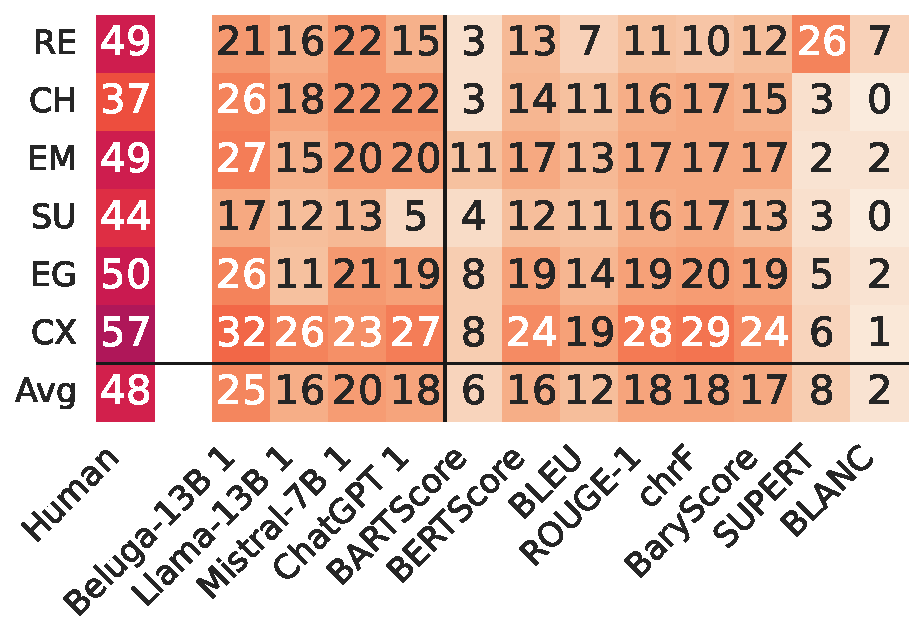
\includegraphics[width=0.6\columnwidth]{pictures/llm_mixed1_story_kendall.pdf}
    \caption{Overall absolute Kendall correlations ($\times$100) between evaluation measures and human ratings. Higher is better.}
    \label{fig:story_level_kendall_mixed1_correlations}
    \end{figure}
    \vspace*{-0.3cm}
    LLMs perform at least as well as other automatic measures, but correlations remain generally low. Fine-tuning and model size seem to improve performance as Beluga-13B has the highest correlations.
\end{frame}

\begin{frame}{Correlations with Human Judgment}
    \begin{figure}[!h]
    \centering
    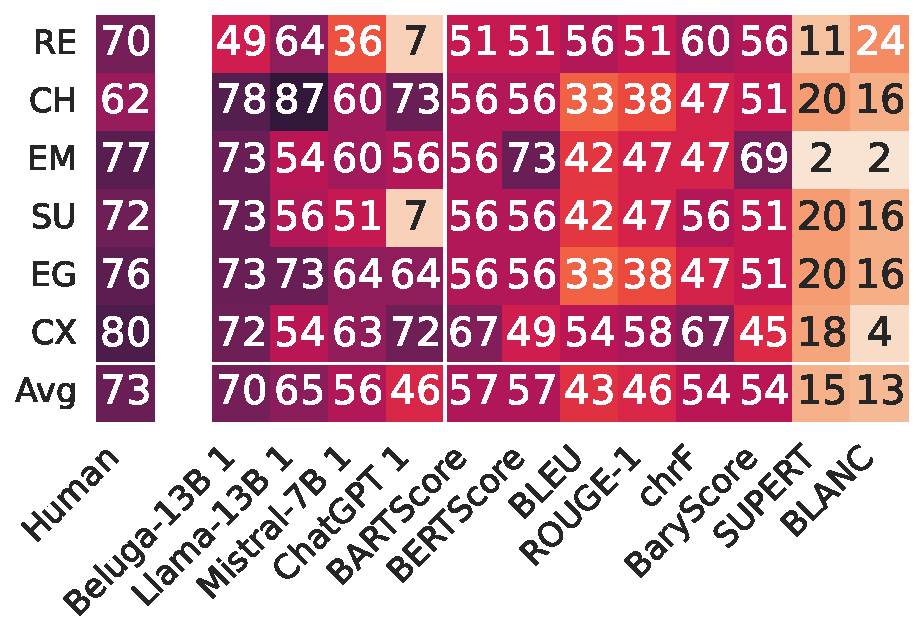
\includegraphics[width=0.6\columnwidth]{pictures/llm_mixed1_w_system_kendall.pdf}
    \caption{System-level absolute Kendall correlations ($\times$100) between evaluation measures and human ratings. Higher is better.}
    \label{fig:system_level_kendall_mixed1_correlations}
    \end{figure}
    \vspace*{-0.3cm}
    Here, LLMs outperform automatic measures. Beluga-13B and Mistral-7B display especially high correlations.
\end{frame}

\begin{frame}{Influence of the Eval-Prompt on Consistency}
    \begin{table}[!h]
        \centering
        \begin{tabular}{lcccc}
        \toprule
        \textbf{Criterion} & \textbf{EP 1} & \textbf{EP 2} & \textbf{EP 3} & \textbf{EP 4} \\
        \midrule
        Relevance & \resultscr{0.88}{0.01} & \resultscr{0.90}{0.01} & \resultscr{0.85}{0.02} & \resultscr{0.92}{0.01} \\
        Coherence & \resultscr{0.93}{0.01} & \resultscr{0.94}{0.01} & \resultscr{0.87}{0.01} & \resultscr{0.93}{0.01} \\
        Empathy & \resultscr{0.88}{0.01} & \resultscr{0.88}{0.01} & \resultscr{0.83}{0.02} & \resultscr{0.91}{0.01} \\
        Surprise & \resultscr{0.80}{0.02} & \resultscr{0.79}{0.02} & \resultscr{0.70}{0.03} & \resultscr{0.85}{0.01} \\
        Engagement & \resultscr{0.91}{0.01} & \resultscr{0.92}{0.01} & \resultscr{0.79}{0.02} & \resultscr{0.93}{0.01} \\
        Complexity & \resultscr{0.85}{0.01} & \resultscr{0.86}{0.01} & \resultscr{0.85}{0.01} & \resultscr{0.89}{0.01} \\
        \bottomrule
        \end{tabular}
        \caption{Intra-class coefficients type 2k for Beluga-13B ratings with 95\% confidence interval. Higher is better.}
        \label{tab:ase2_icc}
    \end{table}
    \vspace*{-0.4cm}
    Providing guidelines (Eval-Prompt 3) appears to slightly decrease consistency with a discernible effect, but ICC values remain very high.
\end{frame}

\begin{frame}{Influence of the Eval-Prompt on Ratings}
    \begin{table}[!h]
        \centering
        \begin{tabular}{lcccc}
        \toprule
        \textbf{LLM} & \textbf{EP 1} & \textbf{EP 2} & \textbf{EP 3} & \textbf{EP 4} \\
        \midrule
        Beluga-13B & \resultscr{3.48}{0.04} & \resultscr{3.38}{0.03} & \resultscr{3.06}{0.03} & \resultscr{3.28}{0.04} \\
        Llama-13B & \resultscr{3.48}{0.03} & \resultscr{3.52}{0.03} & \resultscr{3.21}{0.02} & \resultscr{2.82}{0.03} \\
        Mistral-7B & \resultscr{3.47}{0.03} & \resultscr{3.51}{0.03} & \resultscr{3.46}{0.03} & \resultscr{3.28}{0.03} \\
        \bottomrule
        \end{tabular}
        \caption{Average Likert ratings per LLM per Eval-Prompt. Higher is better.}
        \label{tab:ase2_average}
    \end{table}
     Asking for an explanation (Eval-Prompt 2) has limited influence on ratings, but more detailed Eval-Prompts (3 and 4) tend to decrease the ratings with a statistically discernible effect.
\end{frame}

\begin{frame}{Influence of the Eval-Prompt on Correlations}
    \begin{figure}[!h]
        \centering
        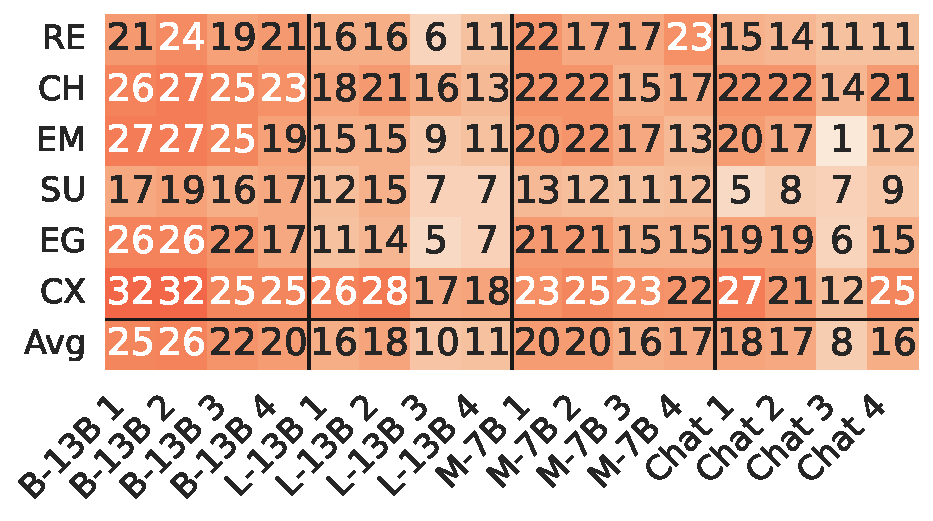
\includegraphics[width=0.7\columnwidth]{pictures/llm_mixed2_story_kendall.pdf}
        \caption{Overall absolute Kendall correlations ($\times$100) between LLMs and human ratings for different Eval-Prompts. Higher is better. B-13B = Beluga-13B, L-13B = Llama-13B, M-7B = Mistral-7B, Chat = ChatGPT.}
        \label{fig:story_level_kendall_mixed2_correlations}
    \end{figure}
    \vspace*{-0.4cm}
    Providing guidelines or a human story (Eval-Prompts 3 and 4) tends to decrease correlations for all models, surprisingly.
\end{frame}

\begin{frame}{Influence of the Eval-Prompt on Correlations}
    \begin{figure}[!h]
        \centering
        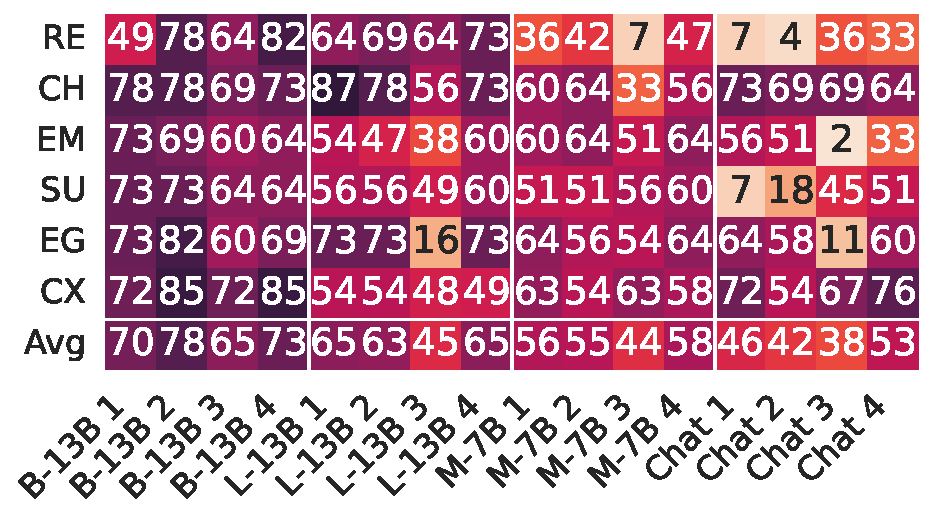
\includegraphics[width=0.7\columnwidth]{pictures/llm_mixed2_w_system_kendall.pdf}
        \caption{System-level absolute Kendall correlations ($\times$100) between LLMs and human ratings for different Eval-Prompts. Higher is better. B-13B = Beluga-13B, L-13B = Llama-13B, M-7B = Mistral-7B, Chat = ChatGPT.}
        \label{fig:system_level_kendall_mixed2_correlations}
    \end{figure}
    \vspace*{-0.4cm}
    Eval-Prompt 3 decreases correlations again, but Eval-Prompt 4 tends to increase them.
\end{frame}

\begin{frame}{Summary}
    \textbf{RQ3: To which extent can we use automatic measures for story evaluation?}
    \begin{itemize}
        \item We performed \textbf{an extensive meta-evaluation}, notably comparing correlations between automatic measures (including LLMs) and human judgment;
        \item Used with prompts based on specific criteria, \textbf{LLMs are currently the best proxy for human evaluation of story generation.} In particular, LLMs display very high system-level correlations with human judgment;
        \item \textbf{LLMs are remarkably self-consistent,} exhibiting very high intra-class coefficient values;
        \item For ASE, \textbf{providing detailed guidelines (Eval-Prompt 3) did not improve correlations with human ratings.} Providing a reference human story (Eval-Prompt 4) yields mixed results;
    \end{itemize}
\end{frame}